%% bare_jrnl_compsoc.tex
%% V1.4a
%% 2014/09/17
%% by Michael Shell
%% See:
%% http://www.michaelshell.org/
%% for current contact information.
%%
%% This is a skeleton file demonstrating the use of IEEEtran.cls
%% (requires IEEEtran.cls version 1.8a or later) with an IEEE
%% Computer Society journal paper.
%%
%% Support sites:
%% http://www.michaelshell.org/tex/ieeetran/
%% http://www.ctan.org/tex-archive/macros/latex/contrib/IEEEtran/
%% and
%% http://www.ieee.org/

%%*************************************************************************
%% Legal Notice:
%% This code is offered as-is without any warranty either expressed or
%% implied; without even the implied warranty of MERCHANTABILITY or
%% FITNESS FOR A PARTICULAR PURPOSE! 
%% User assumes all risk.
%% In no event shall IEEE or any contributor to this code be liable for
%% any damages or losses, including, but not limited to, incidental,
%% consequential, or any other damages, resulting from the use or misuse
%% of any information contained here.
%%
%% All comments are the opinions of their respective authors and are not
%% necessarily endorsed by the IEEE.
%%
%% This work is distributed under the LaTeX Project Public License (LPPL)
%% ( http://www.latex-project.org/ ) version 1.3, and may be freely used,
%% distributed and modified. A copy of the LPPL, version 1.3, is included
%% in the base LaTeX documentation of all distributions of LaTeX released
%% 2003/12/01 or later.
%% Retain all contribution notices and credits.
%% ** Modified files should be clearly indicated as such, including  **
%% ** renaming them and changing author support contact information. **
%%
%% File list of work: IEEEtran.cls, IEEEtran_HOWTO.pdf, bare_adv.tex,
%%                    bare_conf.tex, bare_jrnl.tex, bare_conf_compsoc.tex,
%%                    bare_jrnl_compsoc.tex, bare_jrnl_transmag.tex
%%*************************************************************************


% *** Authors should verify (and, if needed, correct) their LaTeX system  ***
% *** with the testflow diagnostic prior to trusting their LaTeX platform ***
% *** with production work. IEEE's font choices and paper sizes can       ***
% *** trigger bugs that do not appear when using other class files.       ***                          ***
% The testflow support page is at:
% http://www.michaelshell.org/tex/testflow/


\documentclass[10pt,conference,onecolumn,compsoc]{IEEEtran}


\usepackage{hyperref}
\usepackage{enumitem}
\setlist[itemize]{leftmargin=3 cm}
\setlist[enumerate]{leftmargin=3cm}



% *** CITATION PACKAGES ***
%
\ifCLASSOPTIONcompsoc
  % IEEE Computer Society needs nocompress option
  % requires cite.sty v4.0 or later (November 2003)
  \usepackage[nocompress]{cite}
\else
  % normal IEEE
  \usepackage{cite}
\fi
% cite.sty was written by Donald Arseneau
% V1.6 and later of IEEEtran pre-defines the format of the cite.sty package
% \cite{} output to follow that of IEEE. Loading the cite package will
% result in citation numbers being automatically sorted and properly
% "compressed/ranged". e.g., [1], [9], [2], [7], [5], [6] without using
% cite.sty will become [1], [2], [5]--[7], [9] using cite.sty. cite.sty's
% \cite will automatically add leading space, if needed. Use cite.sty's
% noadjust option (cite.sty V3.8 and later) if you want to turn this off
% such as if a citation ever needs to be enclosed in parenthesis.
% cite.sty is already installed on most LaTeX systems. Be sure and use
% version 5.0 (2009-03-20) and later if using hyperref.sty.
% The latest version can be obtained at:
% http://www.ctan.org/tex-archive/macros/latex/contrib/cite/
% The documentation is contained in the cite.sty file itself.



% *** GRAPHICS RELATED PACKAGES ***
%
\ifCLASSINFOpdf
   \usepackage[pdftex]{graphicx}
 
\else
 
\fi
% graphicx was written by David Carlisle and Sebastian Rahtz. It is
% required if you want graphics, photos, etc. graphicx.sty is already
% installed on most LaTeX systems. The latest version and documentation
% can be obtained at: 
% http://www.ctan.org/tex-archive/macros/latex/required/graphics/
% Another good source of documentation is "Using Imported Graphics in
% LaTeX2e" by Keith Reckdahl which can be found at:
% http://www.ctan.org/tex-archive/info/epslatex/
%
% latex, and pdflatex in dvi mode, support graphics in encapsulated
% postscript (.eps) format. pdflatex in pdf mode supports graphics
% in .pdf, .jpeg, .png and .mps (metapost) formats. Users should ensure
% that all non-photo figures use a vector format (.eps, .pdf, .mps) and
% not a bitmapped formats (.jpeg, .png). IEEE frowns on bitmapped formats
% which can result in "jaggedy"/blurry rendering of lines and letters as
% well as large increases in file sizes.
%
% You can find documentation about the pdfTeX application at:
% http://www.tug.org/applications/pdftex









% *** PDF, URL AND HYPERLINK PACKAGES ***
%
\usepackage{url}
% url.sty was written by Donald Arseneau. It provides better support for
% handling and breaking URLs. url.sty is already installed on most LaTeX
% systems. The latest version and documentation can be obtained at:
% http://www.ctan.org/tex-archive/macros/latex/contrib/url/
% Basically, \url{my_url_here}.




\begin{document}

\title{C\# WPF Video Player}
%
%

% received ..."  text while in non-compsoc journals this is reversed. Sigh.

\author{Zachary Rose, Logan Walsh
}

\IEEEtitleabstractindextext{%
\begin{abstract}
Our project is a custom video player as a C\# WPF application. It will allow you to browse to a file, load up a video, and control the playback as needed. AVI, MWV, and MP4 will be supported file types. Those who want more control over their video playback beyond what Windows comes with will find this application useful. 
\end{abstract}

}


% make the title area
\maketitle


\IEEEdisplaynontitleabstractindextext

\IEEEpeerreviewmaketitle



\section{Introduction}


For this project, we plan to make a media player program that offers some features that are unavailable in Windows Media Player. It will include a file browser to select a media file, and it will include the controls for playback such as: play/pause, fast forward/slow down, and skip to different parts of the video, as well as volume controls. 

This project is intended for those who want some finer control over the playback of their video files. Windows Media Player does have the basic features for controlling playback of media, but it leaves much to be desired in customization and more niche functionality. 

Windows Media Player lacks features such as moving forward and backwards a frame at a time, enlarging the video at a key press, and muting the video with a key press. In fact, Windows Media Player lacks keyboard controls entirely. VLC Media Player has these features and more, but it can sometimes feel daunting and over bloated for an average use case. This media player will fit comfortably in the middle between the most casual of users and super users. 

\subsection{Background}

Some useful terminology: 
\begin{itemize}
\item media: in this case, a file containing video and/or sound
\item media player: a program that can playback different media, and it usually allows for some control over different aspects of the playback
\item playback: media is in playback when it is currently being shown to the user
\item file browser: a user interface to make selecting a file from the system convenient 
\item Windows Media Player: a media player that comes with Windows OS by default. Very bare-bones. 
\item Fullscreen: refers to when the video is scaled up to cover an entire monitor. 
\end{itemize}

We decided to make a media player because we thought it would be interesting to make a tool that we might actually use, rather than some project for the sake of displaying some unusual programming concept. It will be good practice towards developing a user interface for a user-oriented application. 

\subsection{Impacts}

Our hope is that this project will become a useful little tool for those who wish to have a light-weight and customizable media player. 

\subsection{Challenges}

By far the hardest thing will likely be designing an interface to dynamically change key bindings. It will need a file to store them, the ability to parse and edit said file, and an interface with which the user will change the bindings from within the app. 


\section{Scope}

Basic goals for getting started: You can load up a video, play and pause it using buttons, and it can be replayed. 

The project will be done once the program runs without any issues and has enough features to differentiate it from Windows Media Player. In other words, the ability to control the video playback with the keyboard and to create custom keybindings. 

We think that this is a worthwhile project because it has practical use, and it will allow us to make further use of the WPF framework. It will require an attractive interface and different form elements working together behind the scenes. 

Basic Goals:
\begin{itemize}
\item Can load a video file to prepare for playback.
\item Can control playback through both mouse and keyboard. 
\item Supports AVI, MKV, and MP4 filetypes. 
\end{itemize}

Stretch Goals:
\begin{itemize}

\item Permanent customization for key bindings, with the ability to reset to defaults. 
\item Combining multiple files into a playlist with associated skip forward/backwards buttons.
\item WPF window can be resized, with all the elements keeping the same size ratio. 
\end{itemize}

\subsection{Requirements}
The functional requirements for a media player are straight forward for anyone who has used one before. We considered what we want to be able to do when watching a video, as well as what is absolutely necessary to do so. Loading a file is the absolute base requirement, but we've come to expect things like pausing and fast forwarding.

\subsubsection{Functional}
\begin{itemize}
\item User can play video files
\item User can use video timeline to skip to desired part of video directly
\item Application supports fullscreen playback 
\item User can pause and unpause the playback at will
\item Application supports different playback speeds, between .5x and 2x
\item User can change the volume as desired
\end{itemize}


\subsubsection{Non-Functional}
\begin{itemize}
\item Application must be able to edit and reload keybindings between different sessions. 
\item Application must be able to load and play several videos sequentially without performance loss.
\end{itemize}

\subsection{Use Cases}
\begin{itemize}
\item[Use Case Number:] 1
\item[Use Case Name:] Loading up a video
\item[Description:] The user wants to load a video from their hard drive to prepare for playback.
\end{itemize}

\begin{enumerate}
\item User opens up file browsing menu by left-clicking "File," followed by "Load File" (See Figure \ref{FileSearchMockup}).
\item User navigates to desired video and selects it.
\item[Termination Outcome:] Video is loaded and begins playback.
\end{enumerate}

Alternative: User wishes to load a video using a file path
\begin{enumerate}
\item User enters file path into search bar (See Figure \ref{FileSearchMockup}).
\item User left-clicks "OK" button.
\item[Termination Outcome:] Video is paused and prepared for playback.
\end{enumerate}

Note: File selected doesn't exist.
\begin{enumerate}
\item User selects a file that doesn't exist, doesn't have permissions to play, or isn't a valid video format.
\item[Termination Outcome:] Application requests a valid file and allows for re-entry. 

\end{enumerate}
\begin{itemize}
\item[Use Case Number:] 2
\item[Use Case Name:] Editing keybindings
\item[Description:] The user wants to change the default keyboard bindings for different aspects of playback control and expects these changes to persist through different sessions of using the application.
\end{itemize}

\begin{enumerate}
\item User opens up the options by left-clicking the "Options" tab with the mouse.
\item User selects "Hotkeys" by left-clicking with the mouse.
\item User selects the binding they want to change, and presses the desired keyboard key to change it to.
\item[Termination Outcome:] New keybindings are set for any available functionality, and the new bindings will be saved to a file for automatic loading upon opening the application. 
\end{enumerate}

\begin{itemize}
\item[Use Case Number:] 3
\item[Use Case Name:] Controlling playback
\item[Description:] During playback, the user wants to control different aspects of the playback. See Figure \ref{PlayerMockup} for the buttons available to left-click. 
\end{itemize}

\begin{enumerate}
\item User pauses and unpauses playback by left-clicking the pause button. 
\item User increases and decreases playback speed using the corresponding buttons.  
\item Alternative: User enters a playback speed directly into the text box and presses the enter key.
\item User increases and decreases volume by dragging the volume slider using the mouse.
\item User enters fullscreen mode by left-clicking the fullscreen button.
\item[Termination Outcome:] Video is in playback in the way desired by the user.
\end{enumerate}

Alternative: User wishes to use keybindings to control video playback
\begin{enumerate}
\item User pauses and unpauses playback by pressing the bound buttons on the keyboard.
\item User increases and decreases playback speed by pressing the bound buttons on the keyboard.
\item User increases and decreases volume by pressing the bound buttons on the keyboard.
\item User enters fullscreen mode by pressing the bound button on the keyboard.
\item[Termination Outcome:] Video is in playback in the way desired by the user.
\end{enumerate}

\begin{figure}[ht!]
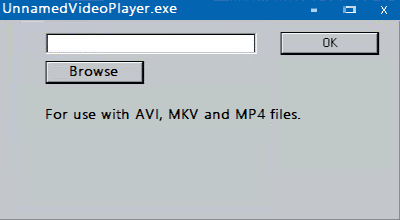
\includegraphics[height=250px, width=350px]{FileSearchMockup.png}
\caption{Sample of interface for selecting video file}
\label{FileSearchMockup}
\end{figure}

\begin{figure}[ht!]
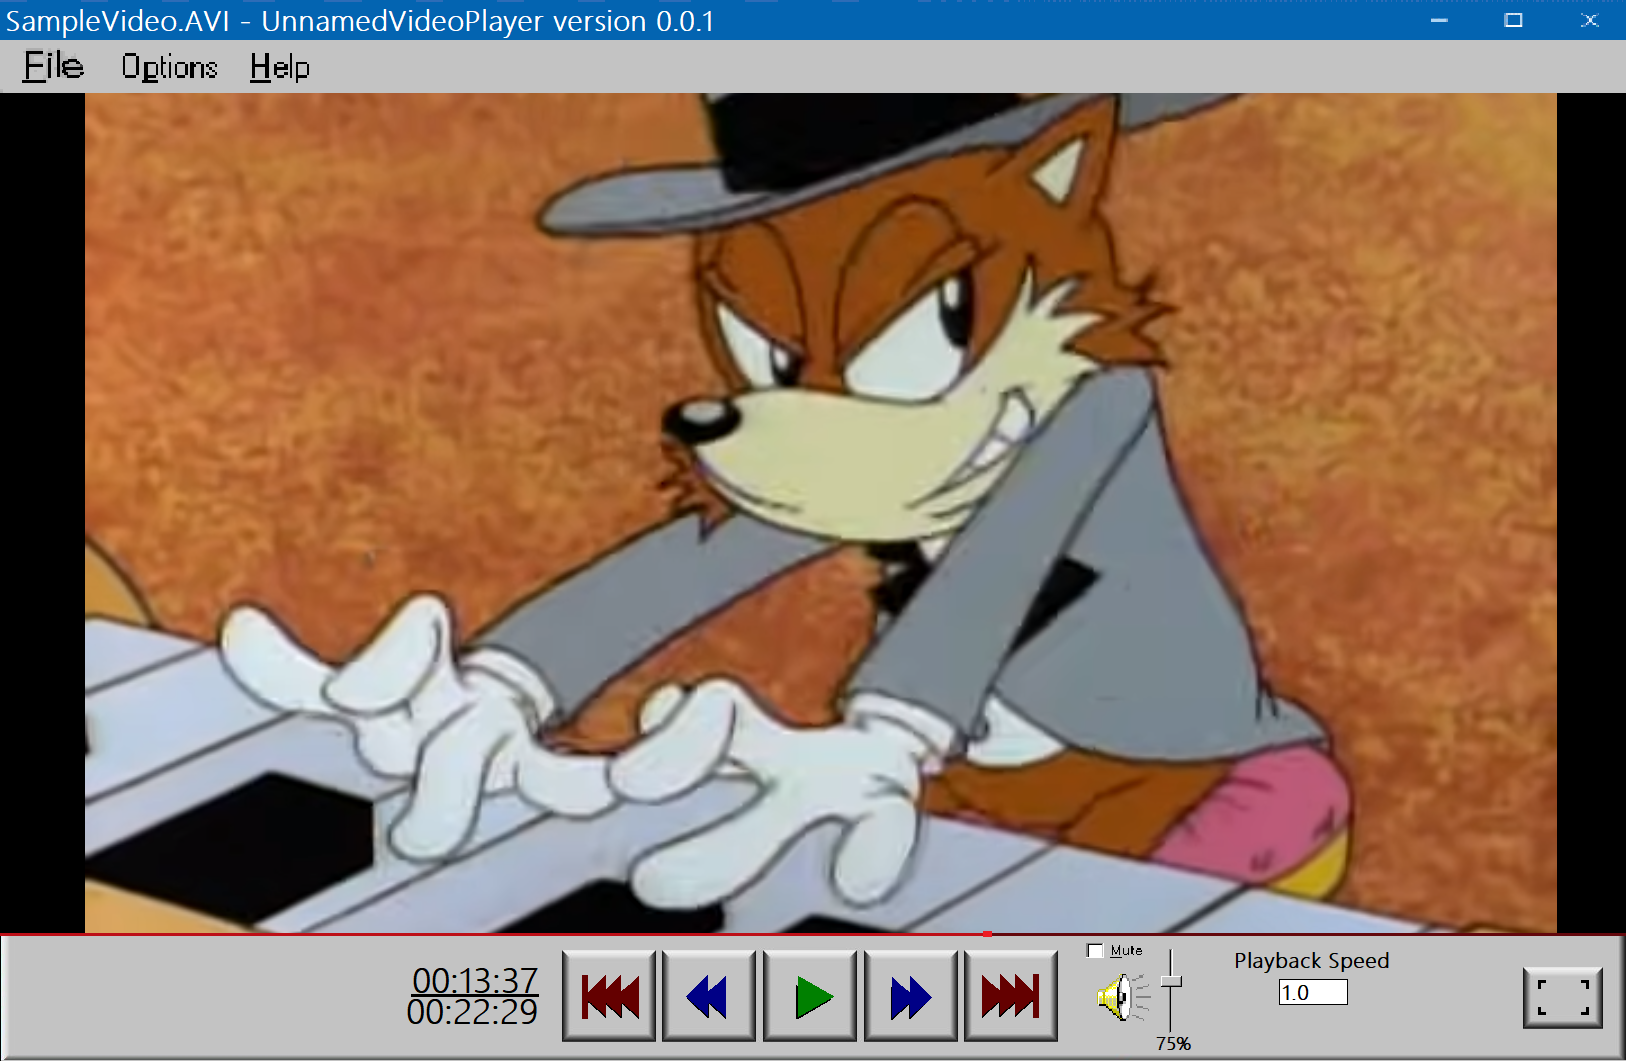
\includegraphics[height=250px, width=350px]{PlayerMockup.png}
\caption{Sample of interface when a video is in playback}
\label{PlayerMockup}
\end{figure}

\subsection{Interface Mockups}
At first, this will largely be completely made up, as you get further along in your project, and closer to a final product, this will typically become simple screenshots of your running application.

In this subsection, you will be showing what the screen should look like as the user moves through various use cases (make sure to tie the interface mockups back to the specific use cases they illustrate).



\section{Project Timeline}
Go back to your notes and look up a typical project development life cycle for the Waterfall approach.  How will you follow this life cycle over the remainder of this semester?  This will usually involve a chart showing your proposed timeline, with specific milestones plotted out.  Make sure you have deliverable dates from the course schedule listed, with a plan to meet them (NOTE: these are generally optimistic deadlines).

( Make a graph)
By April 21th, coding phase should be mostly done.
->April 26th: Testing Phase 
April 27th: Final presentation

\section{Project Structure}
At first, this will be a little empty (it will need to be filled in by the time you turn in your final report).  This is your chance to discuss all of your design decisions (consider this the README's big 
brother).

Our main class contains several important features that work together to update the Media Element. A seeker is updated on a timer to remain updated with video playback, and in the same way the video playback is updated when the seeker is moved. A timer is also used to implement playing in reverse; every tick of the timer pushes the media backwards by an amount with respect to the video playback speed. 

A Factory class is used to change the appearance of the application during runtime. This was chosen in order to simplify adding more themes by keeping them unbound from the main class.

\subsection{UML Outline}
Show the full structure of your program.  Make sure to keep on updating this section as your project evolves (you often start out with one plan, but end up modifying things as you move along).  As a note, while Dia fails miserably at generating pdfs (probably my fault), I have had much success with png files.  Make sure to wrap your images in a \texttt{figure} environment, and to reference with the \texttt{ref} command.  For example, see Figure \ref{cat2}.

\begin{figure}[ht!]
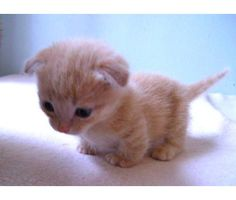
\includegraphics[scale=1.5]{cat2.jpg}
\caption{Your figures should be in the \emph{figure} environment, and have captions.  Should also be of diagrams pertaining to your project, not random internet kittens}
\label{cat2}
\end{figure}


\subsection{Design Patterns Used}
Make sure to actually use at least 2 design patterns from this class.  This is not normally part of such documentation, but largely just specific to this class -- I want to see you use the patterns!


\section{Results}
This section will start out a little vague, but it should grow as your project evolves.  With each deliverable you hand in, give me a final summary of where your project stands.  By the end, this should be a reflective section discussing how many of your original goals you managed to attain/how many desired use cases you implemented/how many extra features you added.

\subsection{Future Work}
Where are you going next with your project?
For early deliverables, what are your next steps?  (HINT: you will typically want to look back at your timeline and evaluate: did you meet your expected goals?  Are you ahead of schedule?  Did you decide to shift gears and implement a new feature?)
By the end, what do you plan on doing with this project?  Will you try to sell it?  Set it on fire?  Link to it on your resume and forget it exists?




\begin{thebibliography}{1}

\bibitem{IEEEhowto:kopka}
H.~Kopka and P.~W. Daly, \emph{A Guide to \LaTeX}, 3rd~ed.\hskip 1em plus
  0.5em minus 0.4em\relax Harlow, England: Addison-Wesley, 1999.

\end{thebibliography}



\begin{IEEEbiography}{Michael Shell}
Biography text here.
\end{IEEEbiography}

% if you will not have a photo at all:
\begin{IEEEbiographynophoto}{John Doe}
Biography text here.
\end{IEEEbiographynophoto}

% insert where needed to balance the two columns on the last page with
% biographies
%\newpage

\begin{IEEEbiographynophoto}{Jane Doe}
Biography text here.
\end{IEEEbiographynophoto}





% that's all folks
\end{document}


